\chapter{Análisis}
\section{Arquitectura general}


\begin{figure}[!ht]
	\centering
	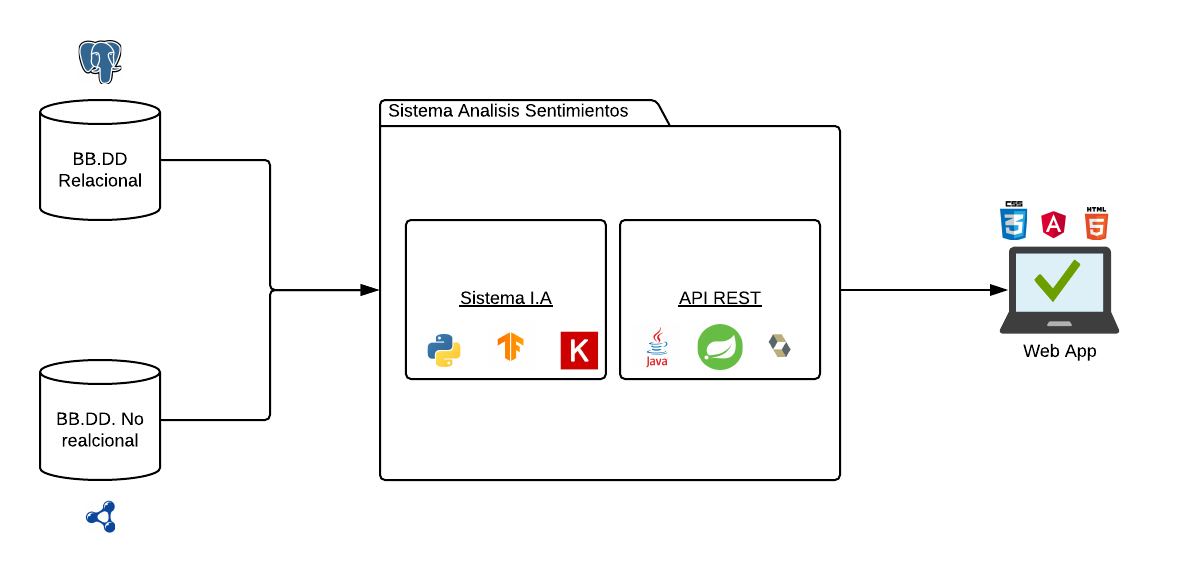
\includegraphics[width=1\textwidth]{imaxes/arqGeneral.png}
	\caption{Arquitectura general del sistema}
	\label{arqGen}
\end{figure}

Como vemos en la figura anterior el sistema se compone de un componente principal que incluye el sistema de inteligencia artificial (clasificación de comentarios) y un sistema que publica una API rest para poder comunicarse con los usuarios finales a través de una aplicación web.

Este sistema se vale de dos bases de datos:
\begin{itemize}
 \item BB.DD relacional: Se almacenan datos de artículos, usuarios y comentarios de forma que se puedan relacionar entre sí.
 \item BB.DD no relacional: Se trata de una base de datos documental con datos sobre las características de los artículos como el color o el material. Se almacena en forma de tripletas RDF y se utiliza en el proceso de búsqueda, el cual queda fuera del alcance de esta memoria.
\end{itemize}

\section{Arquitectura sistema de análisis de sentimientos}

\begin{figure}[H]
	\centering
	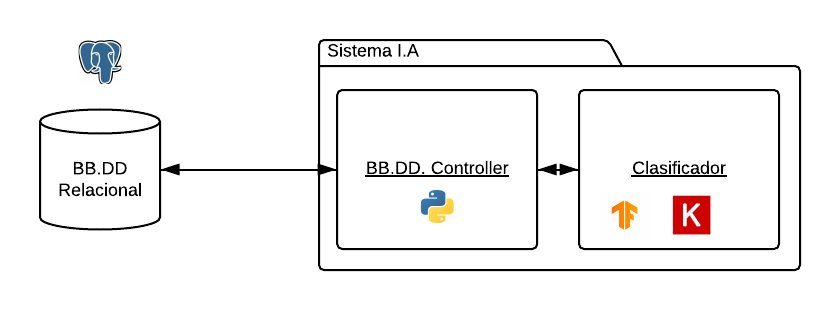
\includegraphics[width=1\textwidth]{imaxes/arqAI.png}
	\caption{Arquitectura del sistema de análisis de sentimientos}
	\label{arqAI}
\end{figure}

\begin{figure}[H]
	\centering
	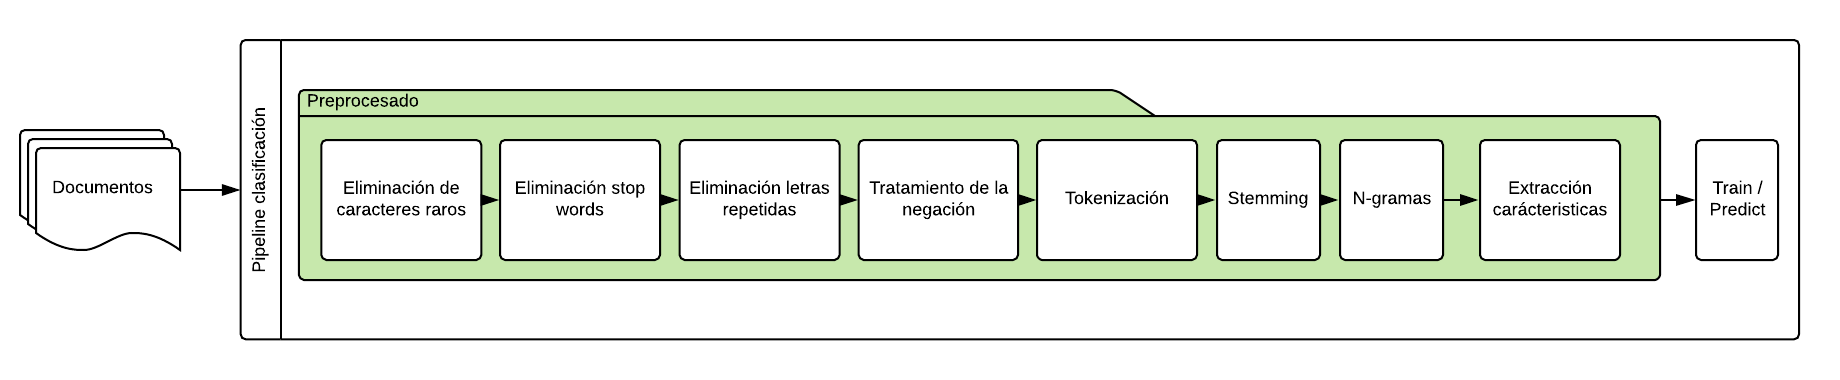
\includegraphics[width=1\textwidth]{imaxes/pipeclasif.png}
	\caption{Arquitectura del clasificador}
	\label{clasifPipe}
\end{figure}

El sistema de clasificación de comentarios (\ref{arqAI}) se compone de dos módulos:

\begin{itemize}
\item Un módulo para gestionar la obtención y actualización de comentarios con la base de datos.
\item Un módulo para realizar la clasificación (\ref{clasifPipe}): Compuesto por un pipeline con dos pasos principales, preprocesado y clasificación o entrenamiento. Los pasos del preprocesado no serán obligatorios y deberán activarse o desactivarse según lo que resulte más conveniente para obtener unos mejores resultados.
\end{itemize}

\section{Arquitectura Web}

\begin{figure}[H]
	\centering
	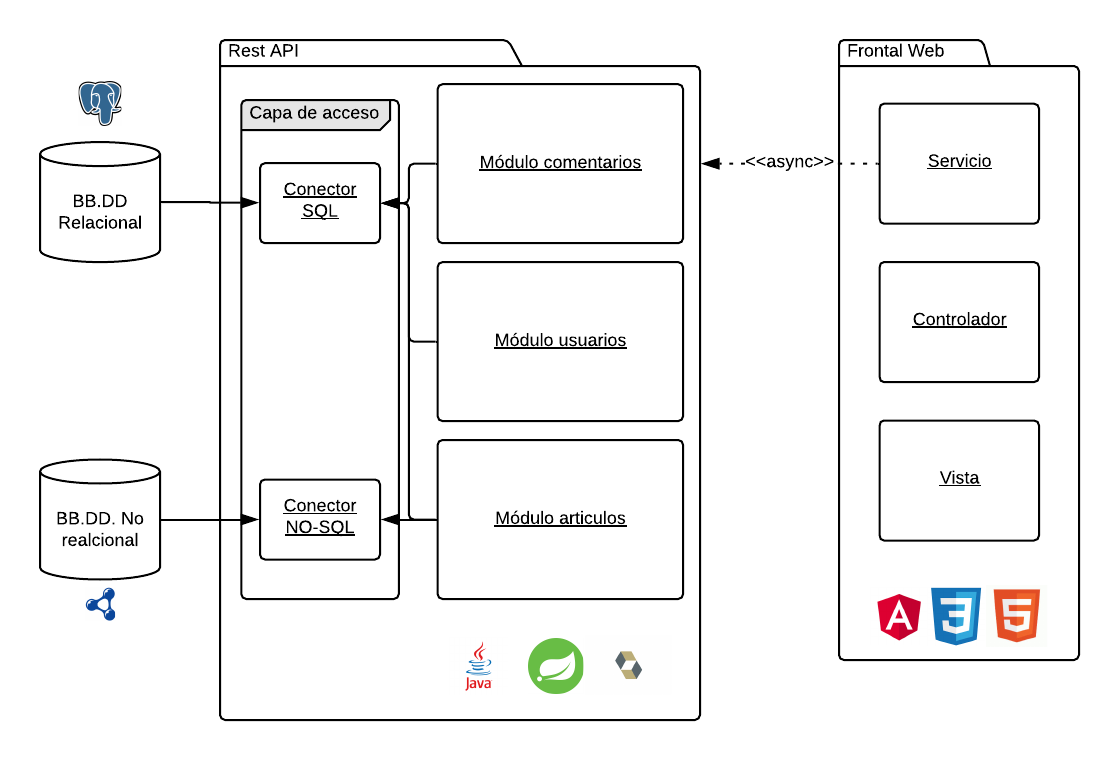
\includegraphics[width=1\textwidth]{imaxes/arqServ.png}
	\caption{Arquitectura del servicio y frontal web.}
	\label{arqServ}
\end{figure}

\begin{figure}[H]
	\centering
	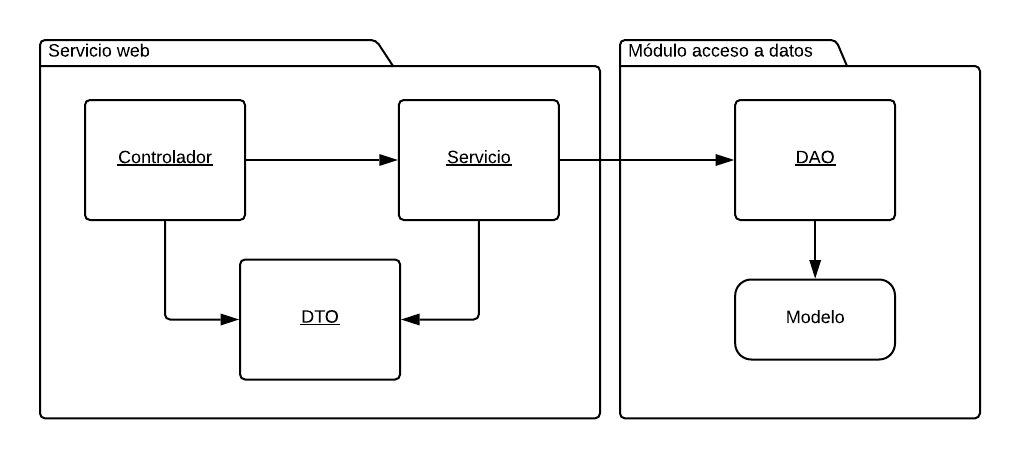
\includegraphics[width=0.75\textwidth]{imaxes/restmodel.png}
	\caption{Ejemplo de arquitectura de un módulo REST del servicio.}
	\label{restModel}
\end{figure}

La aplicación REST (\ref{arqServ}) se compone de tres módulos diferenciados para gestionar las distintas entidades del sistema: usuarios, artículos y comentarios.

Cada módulo sigue un patrón de acceso a datos DAO para abstraerse de la tecnología de base datos utilizada y ser más resistente a cambios, y un patrón DTO para la transmisión de datos, esto nos ayuda a reducir la cantidad de llamadas realizadas al sistema y permite al servicio web abstraerse de la implementación del back-end.

El frontal web se estructura con un patrón MVC (Modelo-Vista-Controlador) en el que el servicio realiza las llamadas asíncronas al API REST y devuelve los datos al controlador, que se encargará de la comunicación entre las vistas y los servicios.

\section{Trabajo futuro} Esta arquitectura se podría simplificar utilizando la nueva librería de javascript TensorflowJS. Con esto podríamos eliminar el sistema de clasificación de comentarios, clasificándolos en caliente en el momento de su publicación desde la aplicación web. 
Para utilizar esta librería solo necesitamos tener un modelo guardado en formato .h5, y dado que la clasificación es un proceso ligero no se espera que suponga una carga importante para el usuario final.
